%%This is a very basic article template.
%%There is just one section and two subsections.
%%This is a very basic article template.
%%There is just one section and two subsections.
\documentclass[a4paper,11pt,oneside,brazilian]{article}

\usepackage[utf8]{inputenx}
\usepackage[brazilian]{babel}
\usepackage{graphicx}
\usepackage{float}
\usepackage{textgreek}
\usepackage{mathtools}
\usepackage{enumerate}
\usepackage{xfrac}

\usepackage{multicol}

\usepackage{pgf,tikz}
\usepackage{pgfplots}
\usepackage{mathrsfs}
\usetikzlibrary{arrows}

\newcommand{\degre}{\ensuremath{^\circ}}
\newcommand{\bfig}{\begin{figure}[!h]\centering}
\newcommand{\efig}{\end{figure}}
\renewcommand{\thesection}{\Roman{section}}


\definecolor{zzttqq}{rgb}{0.6,0.2,0}
\definecolor{xdxdff}{rgb}{0.49,0.49,1}
\definecolor{qqqqff}{rgb}{0,0,1}
\definecolor{cqcqcq}{rgb}{0.75,0.75,0.75}
\definecolor{uuuuuu}{rgb}{0.27,0.27,0.27}
\definecolor{uququq}{rgb}{0.25,0.25,0.25}
\definecolor{qqwuqq}{rgb}{0.0,0.39215686274509803,0.0}
\definecolor{ffqqqq}{rgb}{1.0,0.0,0.0}
\definecolor{ffffff}{rgb}{1,1,1}

\pgfplotsset{compat=1.9}
\begin{document}

\title{Exame Classificatório}
%\author{Matemática}
\date{PVNC 2016}
\maketitle


\begin{flushright}
\emph{Data da realização:} fev/2016
\end{flushright}

\section{Matemática}
\begin{enumerate}[{A}1]
  
  \item Calcule:
  
  \[\frac{1}{3} + \frac{1}{6} = ?\]
  
%   \nopagebreak[4]
% 
% \begin{figure}[H]
% \centering
% 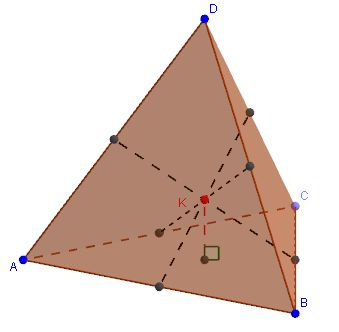
\includegraphics[width=0.9\columnwidth]{tetra.jpg}
% \label{fig:cube}
% \end{figure}
%\nopagebreak[4]
\item Quanto é 16\% de 25?

\item Um cubo de neodímio é um cubo formado por varios pequenos ímãs esféricos
(feitos de neodímio). Um desses cubos está representado na figura abaixo, onde a
aresta do cubo é formada por seis dessas pequenas esferas. Quantas esferas são
necessárias para formar o cubo?

	\begin{figure}[H]
		\centering
		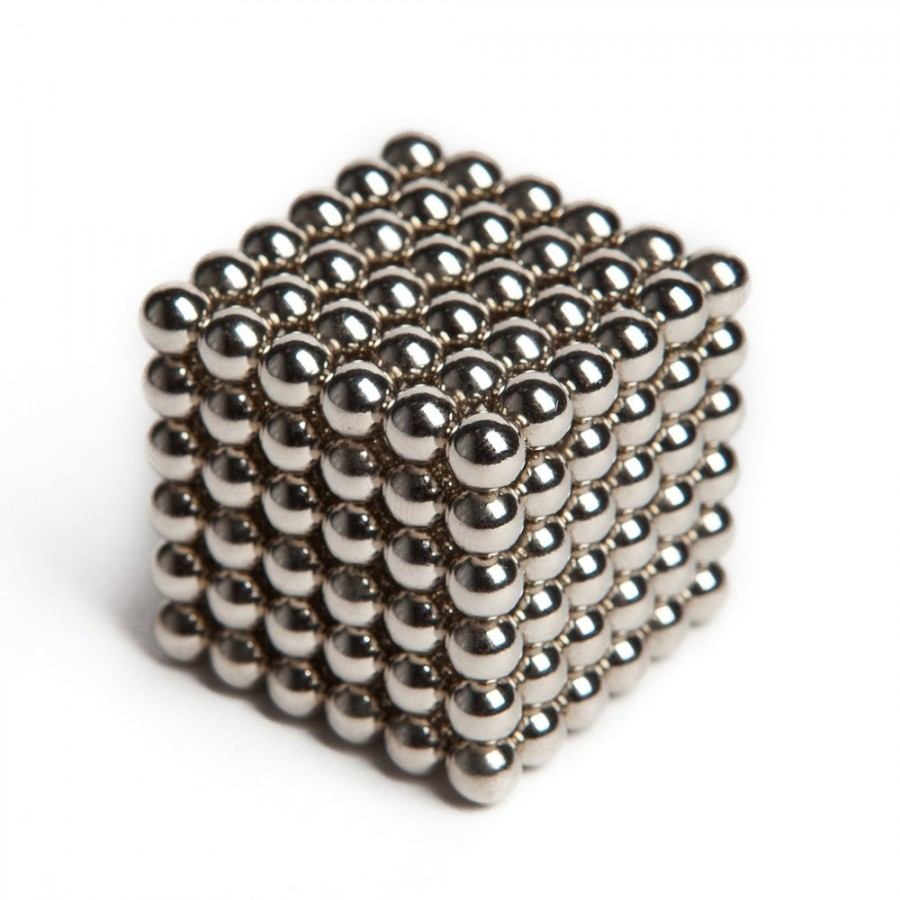
\includegraphics[width=0.7\columnwidth]{neocubes}
	\end{figure}

\item A reta desenhada no plano cartesiano abaixo é a representação gráfica da
seguinte função:
\[y = 2x - 1\]
Determine os pares $(x,y)$ dos pontos $A$ e $B$.

\begin{figure}[!h]
\centering
\begin{tikzpicture}[scale = 2.5, line cap=round,line join=round,>=triangle
45,x=1.0cm,y=1.0cm] \draw[->,color=black] (-0.4970540402756414,0.) -- (1.3142216324462452,0.);
\foreach \x in {,0.5,1.}
\draw[shift={(\x,0)},color=black] (0pt,2pt) -- (0pt,-2pt);
\draw[->,color=black] (0.,-1.2539089632862903) -- (0.,1.2515082846104424);
\foreach \y in {-1.,-0.5,0.5,1.}
\draw[shift={(0,\y)},color=black] (2pt,0pt) -- (-2pt,0pt) node[left] {\footnotesize $\y$};
\draw[color=black] (0pt,-10pt) node[right] {\footnotesize $0$};
\clip(-0.4970540402756414,-1.2539089632862903) rectangle (1.3142216324462452,1.2515082846104424);
\draw [domain=-0.4970540402756414:1.3142216324462452] plot(\x,{(-1.--2.*\x)/1.});
\draw [dash pattern=on 1pt off 1pt] (1.,0.)-- (1.,1.);
\draw (0.9725738259148714,0.04218350911050432) node[anchor=north west] {$1$};
\begin{scriptsize}
\draw [fill=uuuuuu] (0.5,0.) circle (1.0pt);
\draw[color=uuuuuu] (0.5495813035426943,-0.07169909306661988) node {$A$};
\draw [fill=black] (1.,1.) circle (0.5pt);
\draw[color=black] (1.1027253712601566,1.0020511560319798) node {$B$};
\end{scriptsize}
\end{tikzpicture}
\end{figure}

\pagebreak[4]
\item Encontre os valores dos ângulos \(\alpha\) e \(\beta\).

\begin{figure}[!h]
\centering
\begin{tikzpicture}[scale=0.8, line cap=round,line join=round,>=triangle
45,x=1.0cm,y=1.0cm] \clip(4.908268772317717,-5.076297238103462) rectangle (11.083176404771429,-0.19777905334722146);
\draw [shift={(5.,-5.)},color=qqwuqq,fill=qqwuqq,fill opacity=0.1] (0,0) -- (0.:0.22743674521008148) arc (0.:35.:0.22743674521008148) -- cycle;
\draw [shift={(11.,-5.)},color=qqwuqq,fill=qqwuqq,fill opacity=0.1] (0,0) -- (110.:0.22743674521008148) arc (110.:180.:0.22743674521008148) -- cycle;
\draw [shift={(9.781430066596215,-1.6520066239467757)},color=qqwuqq,fill=qqwuqq,fill opacity=0.1] (0,0) -- (-145.:0.3411551178151222) arc (-145.:-70.:0.3411551178151222) -- cycle;
\draw [shift={(9.781430066596215,-1.6520066239467757)},color=qqwuqq,fill=qqwuqq,fill opacity=0.1] (0,0) -- (35.00000000000016:0.3411551178151222) arc (35.00000000000016:110.:0.3411551178151222) -- cycle;
\draw [domain=5.0:11.083176404771429] plot(\x,{(-41.781854419201125--3.4414586181062763*\x)/4.91491226573395});
\draw [domain=4.908268772317717:11.0] plot(\x,{(-51.759108672099885--5.63815572471545*\x)/-2.0521208599540124});
\draw (5.,-5.)-- (11.,-5.);
\begin{scriptsize}
\draw[color=qqwuqq] (5.840759427679051,-4.712398445767332) node {$35\textrm{\degre}$};
\draw[color=qqwuqq] (10.46909719270421,-4.632795584943803) node {$70\textrm{\degre}$};
\draw[color=qqwuqq] (9.593465723645394,-2.2674534347589597) node {$\alpha$};
\draw[color=qqwuqq] (10.116570237628583,-1.0392950106245216) node {$\beta$};
\end{scriptsize}
\end{tikzpicture}
\end{figure}

\nopagebreak[4]
\end{enumerate}


\begin{enumerate}[{B}1]
  \item Encontre os valores de \(x\) que satisfazem a equação: \[x^2 = 1\]
  \item Com o objetivo de recobrir uma caixa de bombom com papel de embrulho, 
  uma pessoa mede as dimensões da caixa e obtém os seguintes valores:
  \begin{itemize}
    \item Altura 8 cm
    \item Largura 26 cm
    \item Profundidade 12 cm
  \end{itemize}
  \begin{figure}[H]
	\centering
	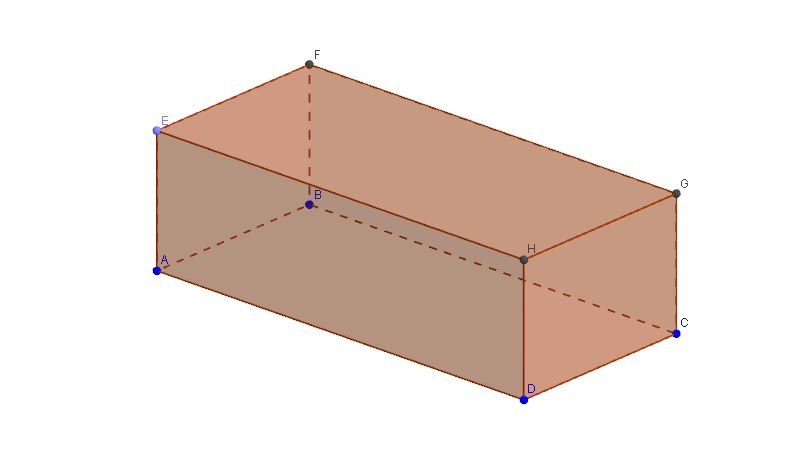
\includegraphics[width=0.9\columnwidth]{prismaretoretangulo.jpg}
	\label{fig:prismaretoretangulo}
	\end{figure}
	
	Determine quantos cm$^2$ de papel a pessoa deve comprar (pelo menos) para que
	seja possível recobrir toda a superfície da caixa de bombom. Considere a caixa
	um paralelepípedo reto como mostra a figura a cima.
	
  \item O que é mais fácil (tem maior probabilidade) uma pessoa lançar 2 vezes
  um dada de 6 faces e tirar 6 nas duas vezes, ou uma pessoa lançar 5 vezes uma
  moeda e tirar cara nas 5 vezes?
	
	
\end{enumerate}
\begin{enumerate}[{C}1]
  \item Um carretel de costura cilíndrico de diâmetro 2 cm é desenrolado sempre
  mantendo a linha esticada. Após desenrolar exatamente uma volta ele se encontra como mostra a figura abaixo.
  \begin{figure}[H]
	\centering
	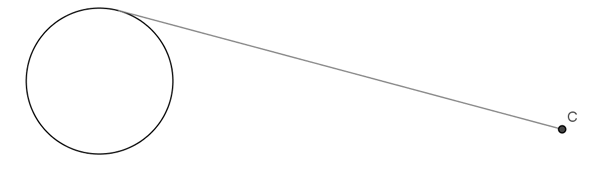
\includegraphics[width=0.9\columnwidth]{carretel.png}
	\label{fig:carretel}
	\end{figure}
  Qual distância da extremidade C da linha até o carretel?
  
\end{enumerate}

\end{document}
